\subsection{Análise Operacional do Cenário de Crise Ambiental (2025)}

Após a otimização arquitetural, a plataforma foi submetida a um cenário extremo de estiagem e incêndios florestais baseados no monitoramento de anomalias térmicas via sensoriamento remoto \cite{giglio_modis_2016}. O sistema permitiu transformar o volume massivo de biometria de calor crua (\textit{raw fire points}) em inteligência tática aplicável à infraestrutura nacional.

\subsubsection{Panorama Geral e Dinâmica nos Biomas}

A crise ambiental atingiu o território nacional de forma aguda e irregular. A Figura \ref{fig:dashboard_outubro} ilustra um painel analítico focado na amostra de outubro de 2025 (pico da estiagem), evidenciando os focos ativos, a área destruída e a severidade do evento (FRP). O painel atesta a macro-evolução do desastre, marcada por um comportamento escalonado e contínuo impulsionado pelo acúmulo agudo das condições de seca.

\begin{figure}[H]
    \centering
    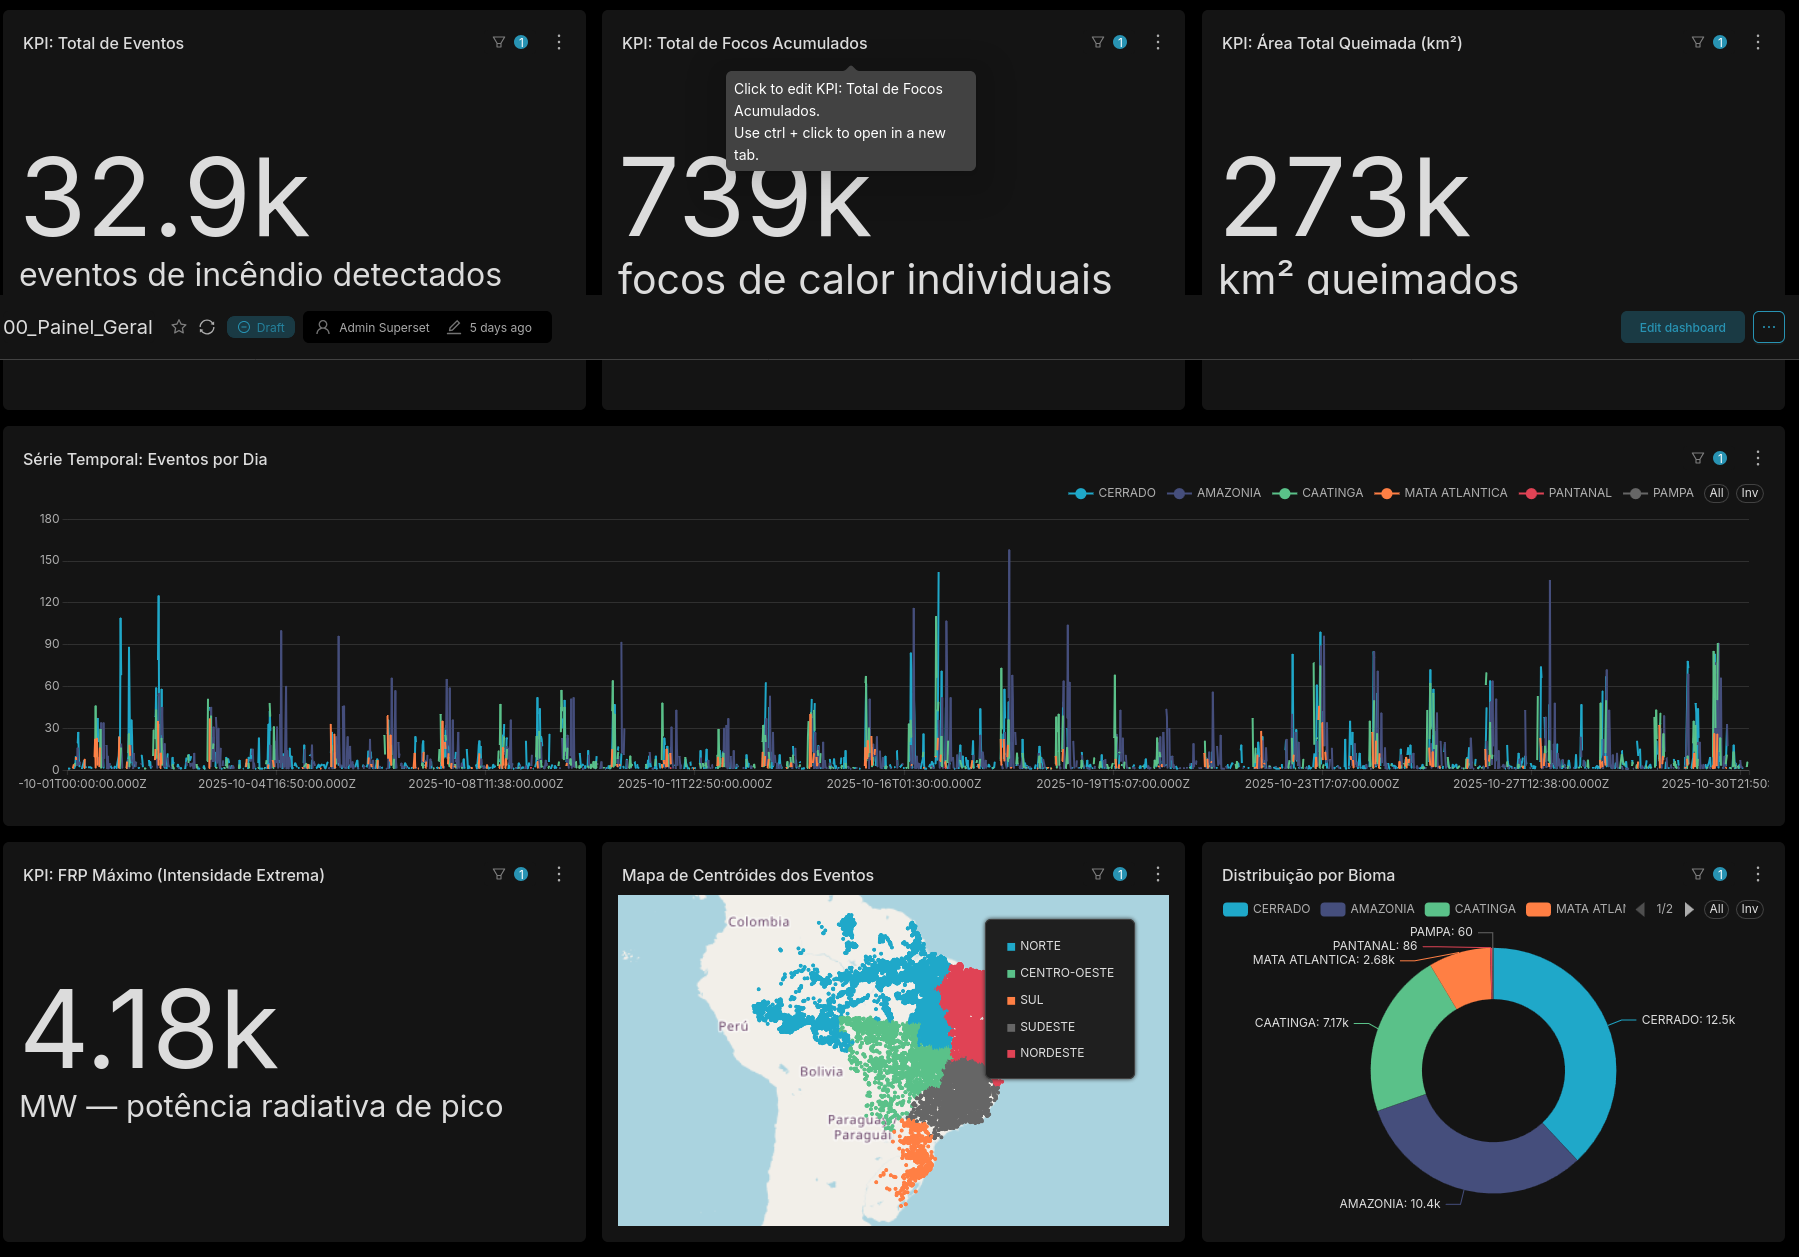
\includegraphics[width=0.9\textwidth]{materiais_apoio/figures/DashBoard.png}
    \caption{Visualização Analítica de Ignições (Apache Superset).}
    \label{fig:dashboard_outubro}
\end{figure}

\subsubsection{Impacto em Comunidades Vulneráveis: Terras Indígenas}

Uma das principais premissas táticas foi mensurar o nível de ameaça sistêmica às comunidades originárias utilizando as malhas poligonais oficiais da FUNAI. O motor analítico rastreou com precisão o cruzamento físico e a aproximação marginal (buffers) das coordenadas de fogo sobre essas demarcações. O resultado prático consolidou um ranking geoespacial de pressão social exibido na Figura \ref{fig:ranking_tis}, revelando os territórios indígenas que apresentaram alta vulnerabilidade espacial.

\begin{figure}[H]
    \centering
    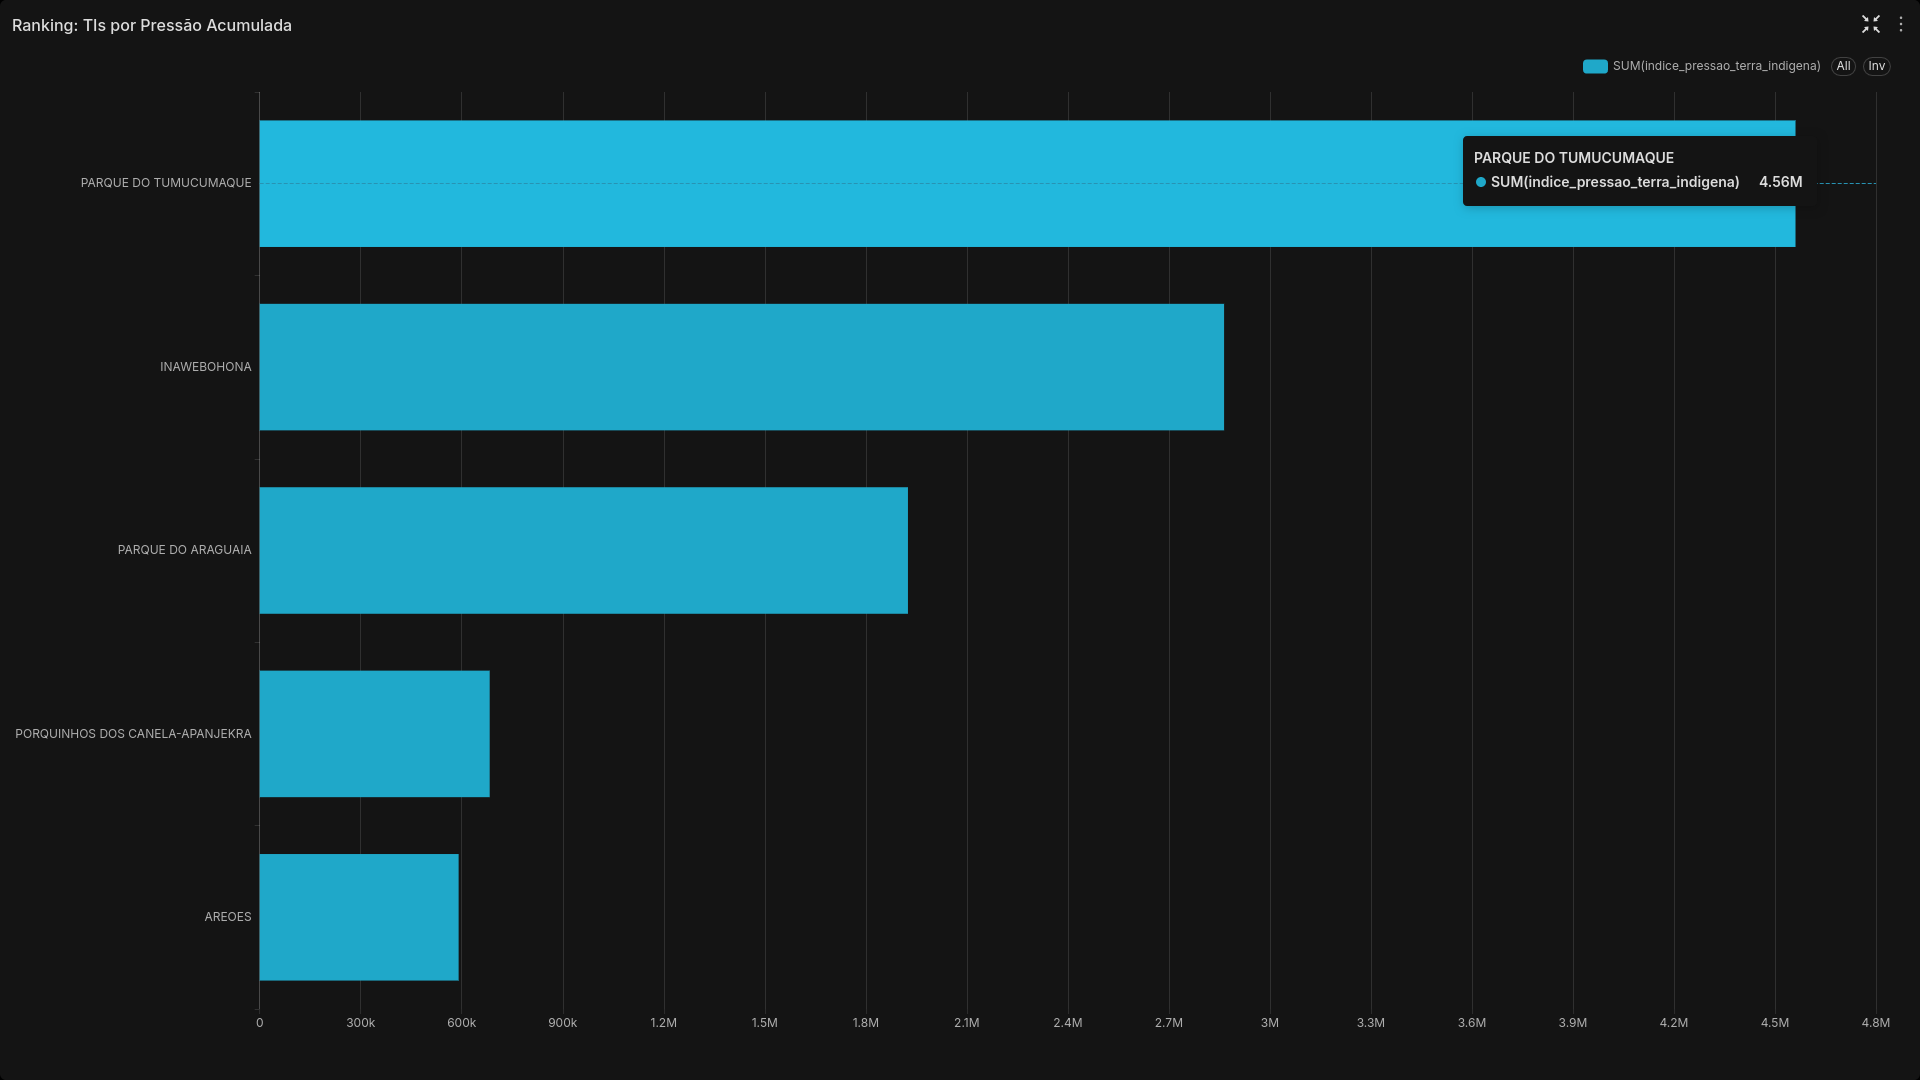
\includegraphics[width=0.9\textwidth]{materiais_apoio/figures/PressãoIndigena.png}
    \caption{Volumetria de Focos em Terras Indígenas.}
    \label{fig:ranking_tis}
\end{figure}

A agregação analítica classificou a \textbf{Terra Indígena Parque do Araguaia} (Formoso do Araguaia/TO) no 3º lugar do ranking de vulnerabilidade com base nos dados de 2025. Levanta-se a hipótese de que essa elevada concentração de anomalias térmicas reflita o avanço do pólo agroindustrial para a porção sul da Ilha do Bananal. Embora o índice calculado não determine causalidade direta para eventos isolados, as métricas parecem corroborar a narrativa cíclica de degradação na região. Segundo reportagem do portal G1, em setembro de 2026, um novo incêndio destruiu 38 residências na Aldeia Canoanã, inserida na mesma demarcação \cite{g1_canoana_2026}. A identificação prévia deste território no topo do ranking sugere que a plataforma pode atuar como um instrumento de apoio para o mapeamento de tendências de exposição e subsidiar ações preventivas.
